\documentclass[9pt]{beamer}
\usepackage{kotex}
\usepackage{amsfonts,amssymb,amsthm}
\usepackage[dvipsnames]{xcolor}
\usepackage{xcolor}
\usepackage{etoolbox}
\usepackage{braket}
\usepackage{tikz}
\usepackage{verbatim}

%## tree 
\usetikzlibrary{trees}
% Set the overall layout of the tree
\tikzstyle{level 1}=[level distance=3.5cm, sibling distance=3.5cm]
\tikzstyle{level 2}=[level distance=3.5cm, sibling distance=2cm]

% Define styles for bags and leafs
\tikzstyle{none} = [text width=0em, text centered]
\tikzstyle{bag} = [text width=4em, text centered]
\tikzstyle{end} = [circle, minimum width=3pt,fill, inner sep=0pt]

%## color
\definecolor{customBlack}{HTML}{3B4252}
\definecolor{customBlackGrey}{HTML}{434C5e}
\definecolor{cuatomGrey}{HTML}{4C566A} 
\definecolor{customWhite}{HTML}{ECEFF4} 
\definecolor{customBlue}{HTML}{6082B6}  
\definecolor{customRed}{HTML}{BF616A}
\definecolor{vividauburn}{rgb}{0.58, 0.15, 0.14}


%## Theme & custom
% \usetheme{metropolis}           % Use metropolis theme
% \metroset{block=fill}
\usetheme{moloch} % modern fork of the metropolis theme
\molochset{block=fill}
\setbeamersize{text margin left=5mm, text margin right=5mm}
\setbeamercolor{palette primary}{bg=customBlack}
\setbeamercolor{alerted text}{fg=customRed}
\setbeamercolor{itemize item}{fg=customBlue}
\setbeamercolor{enumerate item}{fg=customBlue}


%## font
\usefonttheme[onlymath]{serif}
% \setbeamerfont{normal text}{size=\small}
% \setbeamerfont{math text}{size=\tiny}


%## Theorem title, numbering
\makeatletter
\setbeamertemplate{theorem begin}
{%
\begin{\inserttheoremblockenv}
{%
\inserttheoremheadfont
\inserttheoremname
\ifx\inserttheoremaddition\@empty\else\ of\ \inserttheoremaddition\fi%
\inserttheorempunctuation
}%
}
\setbeamertemplate{theorem end}{\end{\inserttheoremblockenv}}
\makeatother
\setbeamertemplate{theorems}[numbered]  


%## Custom block
\setbeamercolor{block title}{bg=customBlue, fg=white}
\setbeamercolor{block body}{bg=customWhite, fg=customBlack}
\setbeamercolor{block title alerted}{%
    use={block title, alerted text},
    bg=customRed,
    fg=white
}
\setbeamercolor{block body alerted}{%
    use={block title, alerted text},
    bg=customWhite,
    fg=customBlack
}
\AtBeginEnvironment{definition}{%
    \setbeamercolor{block title}{fg=white,bg=customBlackGrey}
    \setbeamercolor{block body}{fg=customBlack, bg=customWhite}
}
\AtBeginEnvironment{theorem}{%
    \setbeamercolor{block title}{fg=white,bg=customBlackGrey}
    \setbeamercolor{block body}{fg=customBlack, bg=customWhite}
}
\AtBeginEnvironment{corollary}{%
    \setbeamercolor{block title}{fg=white,bg=customBlackGrey}
    \setbeamercolor{block body}{fg=customBlack, bg=customWhite}
}
\AtBeginEnvironment{lemma}{%
    \setbeamercolor{block title}{fg=white,bg=customBlackGrey}
    \setbeamercolor{block body}{fg=customBlack, bg=customWhite}
}


%! Useful command
% \renewcommand{\Pr}{\text{Pr}}
% $\ast$ \underline{Proof}:
%\checkmark \underline{meaning}:

\title{3. Data Compression, AEP and Lossless Source Coding}
\date{\today}
\author{Vaughan Sohn}
% \institute{Centre for Modern Beamer Themes}


\begin{document}
    %#################################### 
    \maketitle
    
    %#################################### 
    \begin{frame}
        \frametitle{Contents}
        \tableofcontents
    \end{frame}

    
    %#################################### 
    \begin{section}{Source coding}
        \begin{frame}{Communication System}
            Communication system을 표현할 때, 정보이론에서는 "Shannon"이 제안한 \textit{digital communication}을 따른다.
            \begin{itemize}
                \item Shannon의 아이디어는 source와 channel을 나타낼 때, 일관되는 하나의 양식인 binary representation을 따르게 하는 것이다.
                \item Interface를 이용하면, source data의 종류나 channel의 물리적 특성에 관계없이 encoder/decoder만 잘 설계하면 동일한 framework를 적용할 수 있다!
                \item 이번 챕터에서는 "Source coding"에 대해 다루고자 한다.
            \end{itemize}
            \begin{figure}
                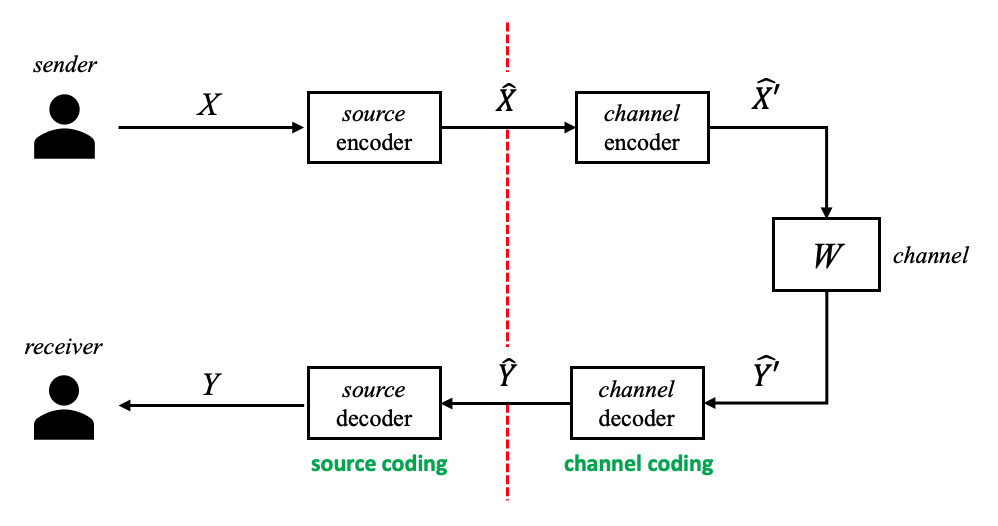
\includegraphics[width=0.7\columnwidth]{image/transmission_system_overview.png}
            \end{figure}
        \end{frame}

        \begin{frame}{Communication System}
            \textbf{Source coding}
            \\ Source coding은 크게 2가지로 이루어져 있다. 
            \begin{itemize}
                \item source encoder: source data를 bit string으로 encoding한다.
                \item source decoder: encoded data를 다시 source data로 decoding한다.
            \end{itemize}
            \begin{alertblock}{Question}
                어떻게 해야 "좋은 encoder"를 설계할 수 있는가?
            \end{alertblock}
            \vspace{0.6cm}
            Source data가 다음의 특성을 가진다고 가정하자.
            \begin{itemize}
                \item source는 특정 alphabet $\mathcal X$에 속한다.
                \item source sequence는 i.i.d이다.
                \item source는 특정 distribution $P$를 따른다.
            \end{itemize}
            \begin{definition}[Discrete Memoryless Source: DMS]
                A sequence $\{X_i\}_{i=1}^{\infty}$ $\sin i.i.d P$ on $\mathcal X$ is called a \textbf{DMS(P)}
            \end{definition}
        \end{frame}

        \begin{frame}{Fixed-length source coding}
            \begin{definition}[fixed-length code]
                A \textbf{Fixed-length code }is a code where each codeword $C(x)$ is restricted to have the \textit{same block length} $L$.
            \end{definition}
            \begin{figure}
                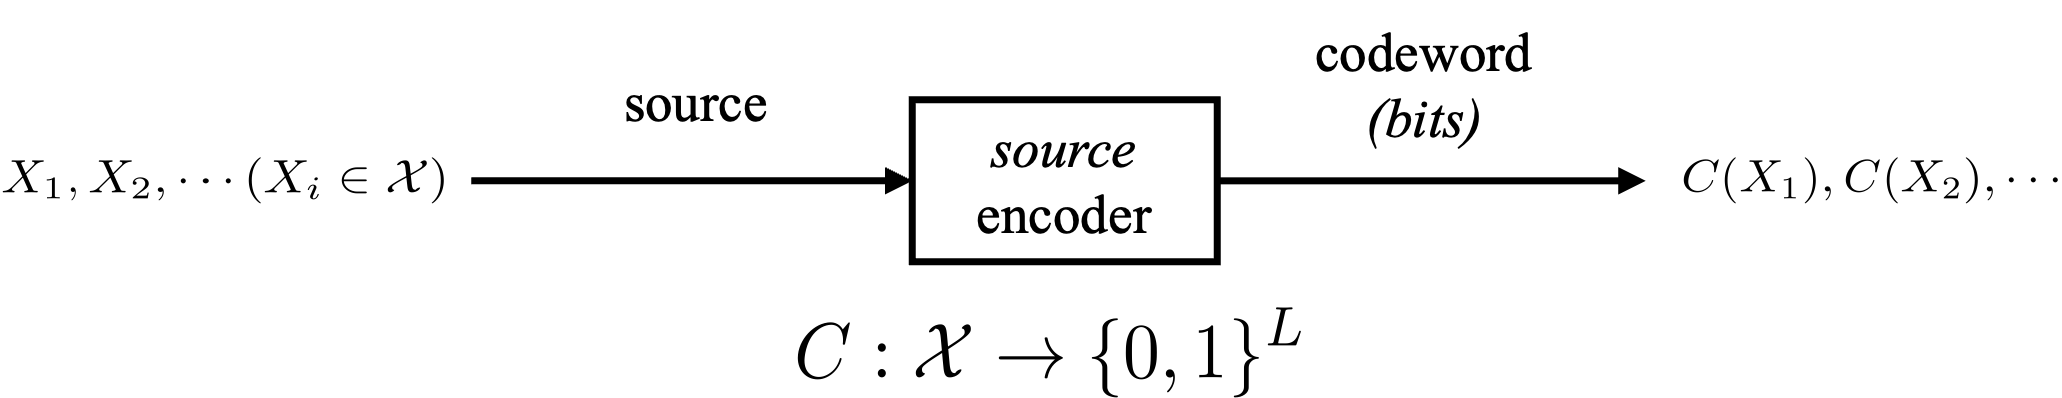
\includegraphics[width=0.8\columnwidth]{image/L3_fixed_length.png}
            \end{figure}
            \begin{itemize}
                \item \textit{Decodability}를 위하여 fixed-length code의 length는 다음 조건을 만족해야한다.
                $$\log M \le L < \log M+1,\qquad (M =|\mathcal X|)$$
                \item Example:
                \\ If the alphabet $\mathcal X$ consists of the 7 symbols $\{a, b, c, d, e, f, g\}$,
                \vspace{1cm}
            \end{itemize}
        \end{frame}

        \begin{frame}{Variable-length source coding}
            \begin{definition}[variable-length code]
                A \textbf{Variable-length code }is a code where each codeword $C(x)$ can have a different length; number of bits $l(x)$ of $C(x)$.
            \end{definition}
            \begin{figure}
                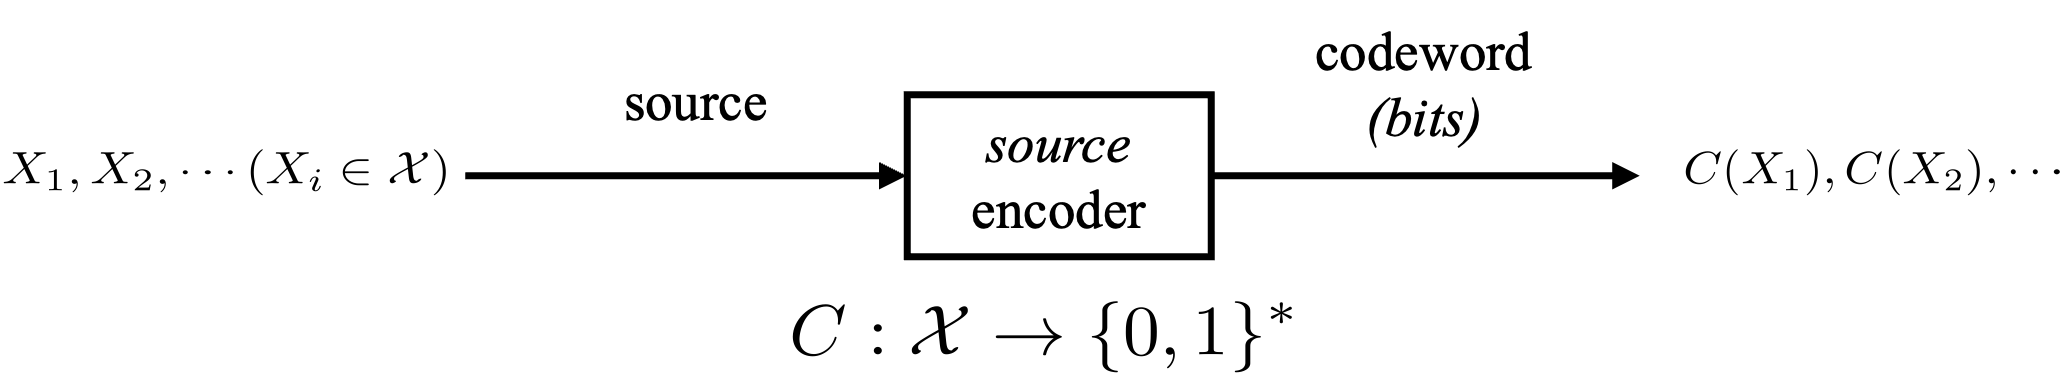
\includegraphics[width=0.8\columnwidth]{image/L3_variable_length.png}
            \end{figure}
            \begin{itemize}
                \item Variable-length code의 length 대한 기댓값 $R$은 다음과 같이 계산할 수 있다.
                $$R = \sum_{x \in \mathcal X} p(x) \cdot l(x)$$
                \item (intuitive) 더 낮은 빈도로 나타나는 symbol에 더 긴 길이의 codeword를 할당하면, expected length of codeword $R$을 줄일 수 있을 것이다.
                \item (problem) 그러나, variable-length code는 fixed-length code와 다르게 어디까지가 하나의 codeword인지를 판단하기 어렵다.
                \\$\rightarrow$\textit{Issue of \alert{decodability!}}
            \end{itemize}
            
        \end{frame}

    \end{section}

    %#################################### 
    \begin{section}{Decodability and optimality}
        \begin{frame}{Uniquely decodable code}
            \begin{definition}[extension]
                The \textbf{extension} $C^*$ of a code $C$ is the mapping from finite-length string of $\mathcal X$ to finite-length string of $\mathcal D = \{0, 1\}$, defined by
                $$C(x_1x_2\cdots x_n) = C(x_1)C(x_2) \cdots C(x_n).$$
            \end{definition}
            \begin{definition}[unique decodability]
                A code is called \textbf{uniquely decodable} if its extension is \textit{non-singular}. In other words, any encoded string in a uniquely decodable code has only one possible source string producing it.
            \end{definition}
            \checkmark \underline{meaning}: extension은 주어진 source data sequence를 codeword sequence로 나타낸 data이다. 만약 이 extension으로부터 다시 원본 source data를 복원할 수 있다면, 그 code는 uniquely decodable이다.
        \end{frame}

        \begin{frame}{Prefix-free code}
            \begin{definition}[prefix-free code]
                A code is called a \textbf{prefix-free code} if no codeword is a \textit{prefix} of any other codeword.
                $$ C(x_j) \notin \{C_1(x_i), C_2(x_i), \cdots, C_n(x_i)\}, \qquad  (\forall i, j, (i\ne j))$$
                where $x_i = b_1b_2\cdots b_n$ and $C_k(x_i) = b_1b_2 \cdots b_k$.
            \end{definition}
            \begin{itemize}
                \item prefix는 어떤 bit string의 initial substring을 의미한다. 
                \item prefix-free code는 어떤 codeword의 prefix도 \textit{자기 자신이 아닌 다른 codeword가 되지 않도록} 설계한 code를 의미한다. 
                \item Example:
                $$
                \begin{aligned}
                    C(a)&=0 & \rightarrow (\text{prefix: }0) \\
                    C(b)&=10 & \rightarrow (\text{prefix: }\{1, 10\})\\
                    C(c)&=11 & \rightarrow (\text{prefix: }\{1, 11\})
                \end{aligned}
                $$
            \end{itemize}

        \end{frame}

        \begin{frame}{Binary-tree representation}
            Source code의 encoding scheme는 binary tree로 표현할 수 있다.
            \begin{itemize}
                \item prefix-free code를 tree로 나타내면, \alert{모든 codeword가 leaf node}에 위치하게 된다.
                \item full tree는 prefix-free 구조를 깨지 않고서는 더이상 새로운 노드를 추가할 수 없는 형태의 tree를 의미한다.
                \item 아래와 같이 $|\mathcal X|=3$에 대해 full tree가 되도록 code를 설계하면, tree의 depth가 줄어들기에 codeword 길이의 기댓값이 줄어든다.
                \begin{figure}
                    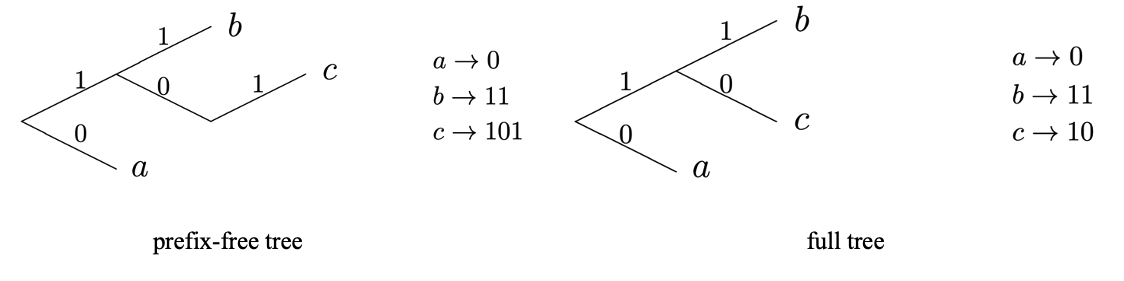
\includegraphics[width=0.75\columnwidth]{image/L3_full_tree_and_prefix_free.png}
                \end{figure}
            \end{itemize}
            \begin{theorem}
                Every prefix-code is uniquely decodable.
                $$ \text{Prefix-free} \subset \text{Uniquely decodable} \subset \text{code} $$
            \end{theorem}
            $\Rightarrow$ Prefix-code의 parsing은 binary-tree에 대한 searching을 \textit{leaf node를 만날 때까지} 수행하면 되기 떄문에 자명하게 uniquely decodable이다.$\Box$
        \end{frame}

        \begin{frame}{Condition of optimal code}
            \begin{lemma}\label{lem:1}
                Optimal codes have the property that if $p_i > p_j$, then $l_i \le l_j$.
            \end{lemma}
            $\ast$ \underline{Proof}: (귀류법) If $p_i > p_j$, then $l_i > l_j$라고 가정하자. 
            \\$\Rightarrow$
            \vspace{0.8cm}
            \begin{lemma}\label{lem:2}
                Optimal prefix-free codes have the property that the associated code tree is \textit{full}.
            \end{lemma}
            $\ast$ \underline{Proof}: 만약 full tree가 아니라면, 언제나 tree depth를 더 줄일 수 있는 다른 full tree를 찾아낼 수 있기 때문에 optimal code가 될 수 없다.$\Box$
            \vspace{0.2cm}
            \begin{lemma}\label{lem:3}
                Two symbols with min. probability have the same length.  In other words, If $p_1 \ge p_2 \ge \cdots \ge p_{M-1} \ge p_M$, then $l_{M-1} = l_M$.
            \end{lemma}
            $\ast$ \underline{Proof}:
            \\By Lemma \ref{lem:1}, if $p_1 \ge p_2 \ge \cdots \ge p_{M-1} \ge p_M$, then $l_1 \le l_2 \le \cdots \le l_{M-1} \le l_M$.
            \\By Lemma \ref{lem:2}, full tree여야 하기 때문에, 가장 확률이 작은 두 노드의 depth는 동일해야한다. $\rightarrow$ sibling node $\Box$
        \end{frame}
    \end{section}

    %#################################### 
    \begin{section}{Huffman Code}
        \begin{frame}
            \frametitle{Huffman Code Algorithm}
            For $X \in \mathcal X$, $X$ be a random symbol with pmf $p_1 \ge p_2 \ge \cdots \ge p_{M-1} \ge p_M$,
            \begin{enumerate}
                \item Choose two least likely symbols ($p_M, p_{M-1}$) and constraining them to be siblings.
                \item Now we consider \textit{new data compression problem} with pmf $\{p_1, p_2, \cdots ,p_{M-2},$ \alert{$p_M + p_{M+1}\}$}
                \item Repeat step 1 \& 2 until there is no more remaining symbol.
            \end{enumerate}
            \vspace{0.5cm}
            Example:

            \begin{figure}
                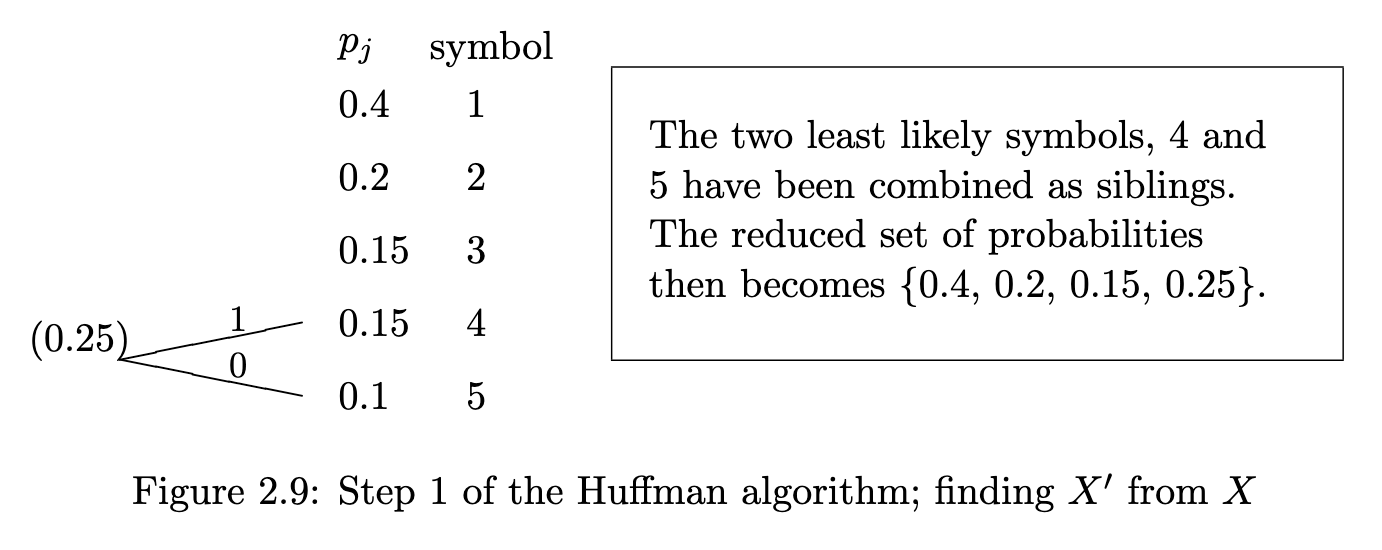
\includegraphics[width=0.8\columnwidth]{image/L3_step1.png}
            \end{figure}
        \end{frame}

        \begin{frame}
            \frametitle{Huffman Code Algorithm}
            For $X \in \mathcal X$, $X$ be a random symbol with pmf $p_1 \ge p_2 \ge \cdots \ge p_{M-1} \ge p_M$,
            \begin{enumerate}
                \item Choose two least likely symbols ($p_M, p_{M-1}$) and constraining them to be siblings.
                \item Now we consider \textit{new data compression problem} with pmf $\{p_1, p_2, \cdots ,p_{M-2},$ \alert{$p_M + p_{M+1}\}$}
                \item Repeat step 1 \& 2 until there is no more remaining symbol.
            \end{enumerate}
            \vspace{0.5cm}
            Example (contd.):

            \begin{figure}
                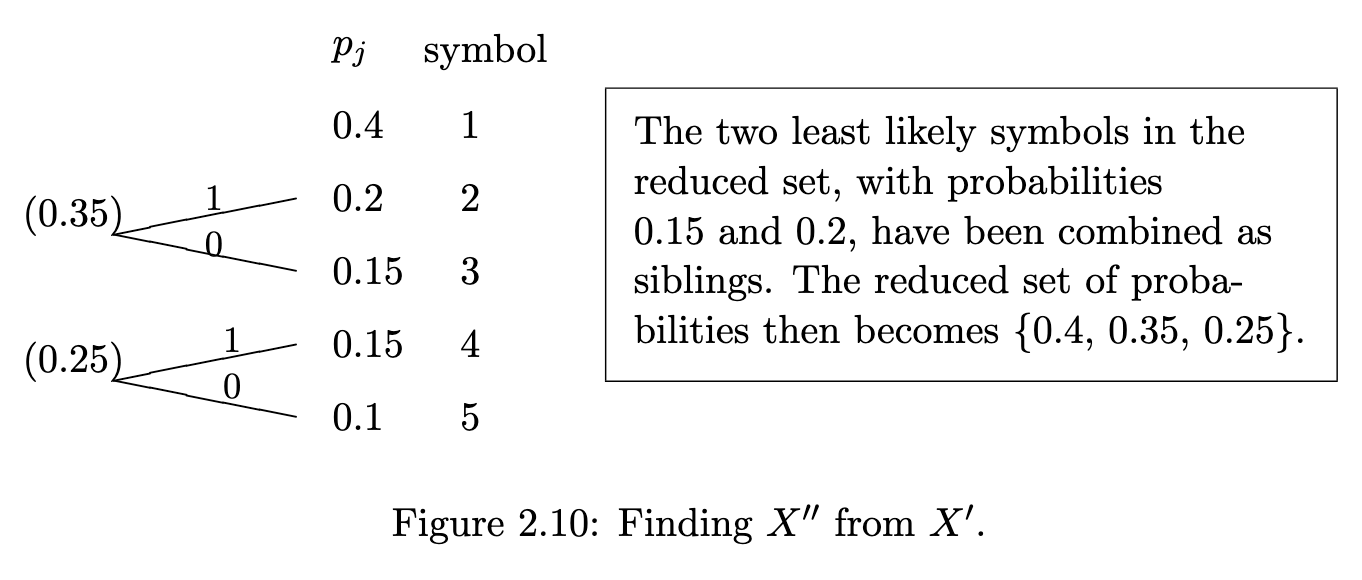
\includegraphics[width=0.8\columnwidth]{image/L3_step2.png}
            \end{figure}
        \end{frame}

        \begin{frame}
            \frametitle{Huffman Code Algorithm}
            For $X \in \mathcal X$, $X$ be a random symbol with pmf $p_1 \ge p_2 \ge \cdots \ge p_{M-1} \ge p_M$,
            \begin{enumerate}
                \item Choose two least likely symbols ($p_M, p_{M-1}$) and constraining them to be siblings.
                \item Now we consider \textit{new data compression problem} with pmf $\{p_1, p_2, \cdots ,p_{M-2},$ \alert{$p_M + p_{M+1}\}$}
                \item Repeat step 1 \& 2 until there is no more remaining symbol.
            \end{enumerate}
            \vspace{0.5cm}
            Example (contd.):

            \begin{figure}
                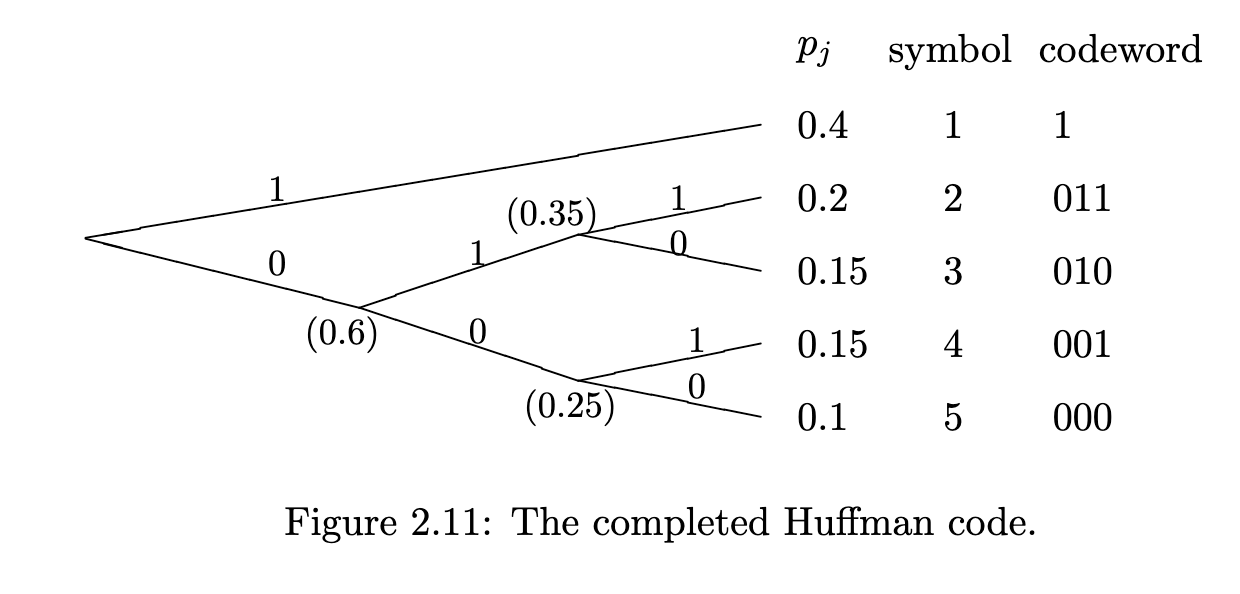
\includegraphics[width=0.75\columnwidth]{image/L3_step3.png}
            \end{figure}
        \end{frame}
        
        \begin{frame}
            \frametitle{Optimality of Huffman code}
            \begin{lemma}
                    Huffman algorithm constructs the \textbf{optimal} prefix-free code. → minimum $R$.
            \end{lemma}
            \vspace{0.2cm}
            $\ast$ \underline{Proof}: $X$에 대한 average length를 $X'=X-\{M-1, M\}\}$에 대한 average length로 표현한 식은 다음과 같다.
            $$R = R' + p_{M-1} + p_M$$
            각 step마다 subproblem $R'$을 minimize하기 때문에, 다음을 이끌어낸다.
            $$R_{min} = R'_{min} + p_{M-1} + p_M$$
            따라서 Huffman algorithm은 optimal이다.$\Box$
        \end{frame}
    \end{section}

    %#################################### 
    \begin{section}{Asmptotic Equipartition Property (AEP)}
        \begin{frame}
            \frametitle{Prerequisites: Weak Law of Large Numbers}
            \begin{theorem}[Weak Law of Large Numbers (WLLN)]\label{thr:WLLN}
                Let $X_1, X_2, \cdots$ be i.i.d with mean $\mu$ and variance $\sigma^2 < \infty$. Let define a new random variable $S_n$ as
                $$S_n \triangleq \frac{1}{n} (X_1 + X_2 + \cdots + X_n).$$
                Then, if $n$ is increasing then $S_n$ convergence to $\mu$.
                $$ S_n \xrightarrow{P} \mu, \quad, \text { i.e., } \quad\left(S_n-\mu\right) \xrightarrow{P} 0 . $$
                In other words, for all $\epsilon, \delta >0$, there exists $N_0$ such that $\forall n > N_0$,
                $$\text{Pr}(|S_n - \mu| > \delta) < \epsilon,$$
                i.e., for all $\delta >0$, 
                $$\lim_{n \rightarrow \infty} \text{Pr} [|S_n - \mu| > \delta ]=0.$$
            \end{theorem}
            \checkmark \underline{meaning}:  Sample의 개수 $n$이 증가할 수록, $S_n$의 값이 $X_i$의 기댓값에 가까워진다는 내용을 다룬다. $n$이 커질수록 variance는 0에 수렴하기 때문에 점점 분포가 sharp해진다.
            $$ \mathbb E[S_n] = \mu, \quad  Var[S_n] = \frac{\sigma^2}{n}$$
        \end{frame}
        
        \begin{frame}
            \frametitle{Prerequisites: Weak Law of Large Numbers}
            For proof of WLLN, we using markov inequality.
            \begin{theorem}[Markov inequality]\label{thr:markov}
                If $Z \ge 0$ and $\gamma > 0$, then
                $$\text{Pr}(Z>\gamma) <  \frac{\mathbb E[Z]}{\gamma}.$$
            \end{theorem}
            \checkmark \underline{meaning}: $[0, \infty)$ 범위에 있는 random variable $Z$에 대해서, $Z$가 특정 값 $\gamma$보다 클 확률은 $\gamma$에 대한 $\mathbb E[Z]$의 비율을 상한으로 가진다.
            \vspace{0.3cm}
            \\$\ast$ \underline{Proof of theorem \ref{thr:markov}}: (hint) $\mathbb E[Z]$를 2개의 event에 대해 decomposition하자.
            $$ \mathbb{E}[Z]=\underbrace{\mathbb{E}[Z | Z>\gamma]}_{} \operatorname{Pr}(Z>\gamma)+\underbrace{\mathbb{E}[Z | Z \leq \gamma] \operatorname{Pr}(Z \leq \gamma)}_{}. $$
            \\$\Rightarrow$
            \vspace{0.5cm}

            $\ast$ \underline{Proof of theorem \ref{thr:WLLN}}: (hint) R.v. $Z \triangleq |S_n - \mu|^2$를 정의하자.
            \\$\Rightarrow$
            \vspace{2cm}
            
        \end{frame}

        \begin{frame}
            \frametitle{Asymptotic Equipartition Property (AEP)}
            \begin{theorem}[Asymptotic Equipartition Property (AEP)]\label{thr:AEP}
                Let $X_1, X_2, \cdots, X_n$ be i.i.d with $P$ over $\mathcal X$. Consider $\boxed{Y_i = -\log P(X_i)}$. Then, by definition of entropy $\mathbb E[Y_i] = H(P)$ ($\ast$). Let us denote $(x_1, x_2, \cdots, x_n)$ by $x_1^n$ or $x^n$.
                \\By applying \textit{WLLN}, $\forall \epsilon, \delta > 0$, $\exists N_0$ such that $\forall n > N_0(\epsilon, \delta)$,
                \\$$ P^n\left[\left\{x_1^n:\left|\underbrace{-\frac{1}{n} \sum_{i=1}^n \log P\left(x_i\right)}_{\text{empirical mean}}-\underbrace{H(P)}_{\text{expectation}}\right|>\delta\right\}\right]<\epsilon $$
            \end{theorem}
            \checkmark \underline{meaning}: Empirical mean과 expectation의 차이가 $\delta$보다 크게 만드는 sequence $x_1^n$들의 집합의 확률은 $\epsilon$보다 작다.
            \begin{itemize}
                \item $P^n$은 확률분포 $P$를 $n$번 곱한 것으로, i.i.d이기 때문에 joint probability가 각 marginal probability들의 곱과 동일하기 때문이다.
                \item $\log$함수의 성질에 의하면, summation of log를 다음과 같이 바꾸어 쓸 수 있다.
                $$ P^n\left[\left\{x_1^n:\left|-\frac{1}{n} \log P^n\left(x_1^n\right)-H(P)\right|>\delta\right\}\right]<\epsilon $$
            \end{itemize}
    
        
        \end{frame}

        \begin{frame}
            \frametitle{Weak typical set}
            \begin{definition}[weak typical set]
                We define \textbf{weak typical set} as,
                $$ A_\delta^{(n)}(P) \triangleq\left\{x_1^n \in \mathcal X^n:\left|-\frac{1}{n} \log P^n\left(x_1^n\right)-H(P)\right| \leq \delta\right\}. $$
            \end{definition}
            \checkmark \underline{meaning}: Empirical mean과 expectation의 차이가 $\delta$보다 작게 만드는 sequence $x_1^n$들의 집합을 weak typical set이라고 정의한다.
            \begin{corollary}
                Theorem \ref{thr:AEP} with typical set $A_{\delta}^{(n)}(P)$ implies that $$ P^n\left(A_\delta^{(n)}(P)\right) \geq 1-\epsilon. $$
            \end{corollary}
            \begin{itemize}
                \item Weak typical set도 $x$의 값에는 영향을 받지않고 그 r.v.가 따르는 확률분포에만 영향받기 때문에 $P$로 표현한다.
                \item 기호의 단순화를 위해 $\delta = \epsilon$으로 두자. $\rightarrow A_{\epsilon}^{(n)}(P)$
            \end{itemize}
            
        \end{frame}   

        \begin{frame}
            \frametitle{Weak typical set}
            $A_{\epsilon}^{(n)}(P)$를 이용하면, weak typical set이 가지는 아주 중요한 성질 하나를 보일 수 있다.
            \begin{itemize}
                \item By definition of weak typical set,
                $$ A_\epsilon^{(n)}(P) \triangleq\left\{x_1^n \in \mathcal X^n:\left|-\frac{1}{n} \log P^n\left(x_1^n\right)-H(P)\right| \leq \epsilon\right\}. $$
                \item set의 elements의 표현에서 절댓값 기호를 제거한 뒤
                $$ = \left\{x_1^n \in \mathcal X^n: -\epsilon \le  -\frac{1}{n} \log P^n\left(x_1^n\right)-H(P) \leq \epsilon\right\},$$
                % Note that nH(P) is the average surprise we get when we observe an arbitrary X_1^.
                \item set의 each element $x_1^n$에 대한 확률에 대해 부등식을 정리하면 다음을 얻는다.
                $$ = \left\{x_1^n: 2^{-n(H(P)+\epsilon)} \leq P^n\left(x_1^n\right) \leq 2^{-n(H(P)-\epsilon)}\right\}$$
            \end{itemize}
            $\Rightarrow$ 즉, weak typical set안에 들어있는 sequence들은 \alert{거의 유사한 확률}을 가진다!
            \vspace{0.3cm}
            \begin{block}{Remarks}
                \begin{itemize}
                    \item 대부분의 sequence들은 weak typical set안에 존재한다.
                    \item typical set안에 있는 sample들의 확률은 거의 동일하다.
                \end{itemize}
            \end{block}

        \end{frame}  

        \begin{frame}
            \frametitle{Weak typical set}
            \begin{corollary}[Size of typical set]
                \begin{itemize}
                    \item For typical set $A_{\epsilon}^{(n)}(P)$,
                    $$ |A_\epsilon^{(n)}(P)| \le 2^{n(H(P)+\epsilon)} $$
                    \item For large enough $n$,
                    $$ |A_\epsilon ^{(n)} (P)| \ge (1-\epsilon) 2^{n{(H(P)-\epsilon)}} $$
                \end{itemize}
            \end{corollary}
            \vspace{0.2cm}
            $\ast$ \underline{Proof}: (hint) sum of probability is 1, and Corollary 16 (with sufficiently large $n$)
            \\$\Rightarrow$
            \vspace{2cm}
        
        \end{frame}  

        \begin{frame}
            \frametitle{With exponential approximation }
            Weak typical set에 대한 더 엄밀한 표현을 위해 exponential approximation을 적용한다.
            \begin{definition}
                For a sequence $f(1), f(2), \cdots, f(n)$ and a constant $c \in \mathbb R$, we say 
                $$f(n) \doteq e^{cn}, \quad iff \quad, \lim_{n \rightarrow \infty} \frac{\log f(n)}{n} = c.$$
                Futhermore, we say  $ f(n) \doteq h(n)$  if both have the same exponential rate, i.e., $f(n) \doteq g(n) \doteq e^{cn}$
            \end{definition}
            \vspace{0.2cm}
            Example: 다음 두 함수가 same exponential rate를 가지는지 확인하라.
            \begin{itemize}
                \item $f(n), cf(n)$
                \item $f(n), n^2 f(n)$
                \item $f(n), f(n)+e^{-n}$
            \end{itemize}
            
            \vspace{0.2cm}
            By exponential approximation, weak typical set은 다음의 성질을 가진다.
            \begin{itemize}
                \item $\forall x_1^n \in A_{\epsilon_n}^{(n)}(P),\ \  P^n\left(x^n\right) \doteq 2^{-n H(P)} .$
                \item The size of set equals $|A_{\epsilon_n}^{(n)}(P)| \doteq 2^{nH(P)}$
                \item $P^n(A_{\epsilon_n}^{(n)}) \rightarrow 1$
            \end{itemize}
        \end{frame}

        \begin{frame}
            \frametitle{Summary }
            \textit{Some Remarks}
            \begin{itemize}
                \item (충분히 큰 $n$에 대하여) sample space $\mathcal X^n$에서 sampling한 data $x^n$은 높은 확률; $P^n \ge 1-\epsilon$로 weak typical set에 포함된다. 
                \item 그러나, 전체 sample space의 크기에 비하여 weak typical set의 크기는 strictly 작다.
                $$ 2^{n H(P)} < 2^{n \log |\mathcal X|} $$
            \end{itemize}
            \vspace{0.2cm}
            \begin{block}{Idea}
                sample space의 전체 data에 대해서 encoding scheme을 설계하는 것보다 typical set에 포함되는 data에 대해서만 encoding scheme를 설계하는 것이 훨씬 더 효과적이다! 
                \\ $\rightarrow$ \textit{Lossless source coding}
            \end{block}
        \end{frame}
    \end{section}

    %#################################### 
    \begin{section}{Loseless source coding}
        \begin{frame}
            \frametitle{Fixed-length block coding}
            \begin{definition}[fixed-length block code]
                A \textbf{Fixed-length block code }is a code where a source block  $x^n$ , consisting of  $n$ symbols from the source alphabet $(x_i \in \mathcal X)$, is represented by a codeword $C(x^n)$.
            \end{definition}
            \begin{figure}
                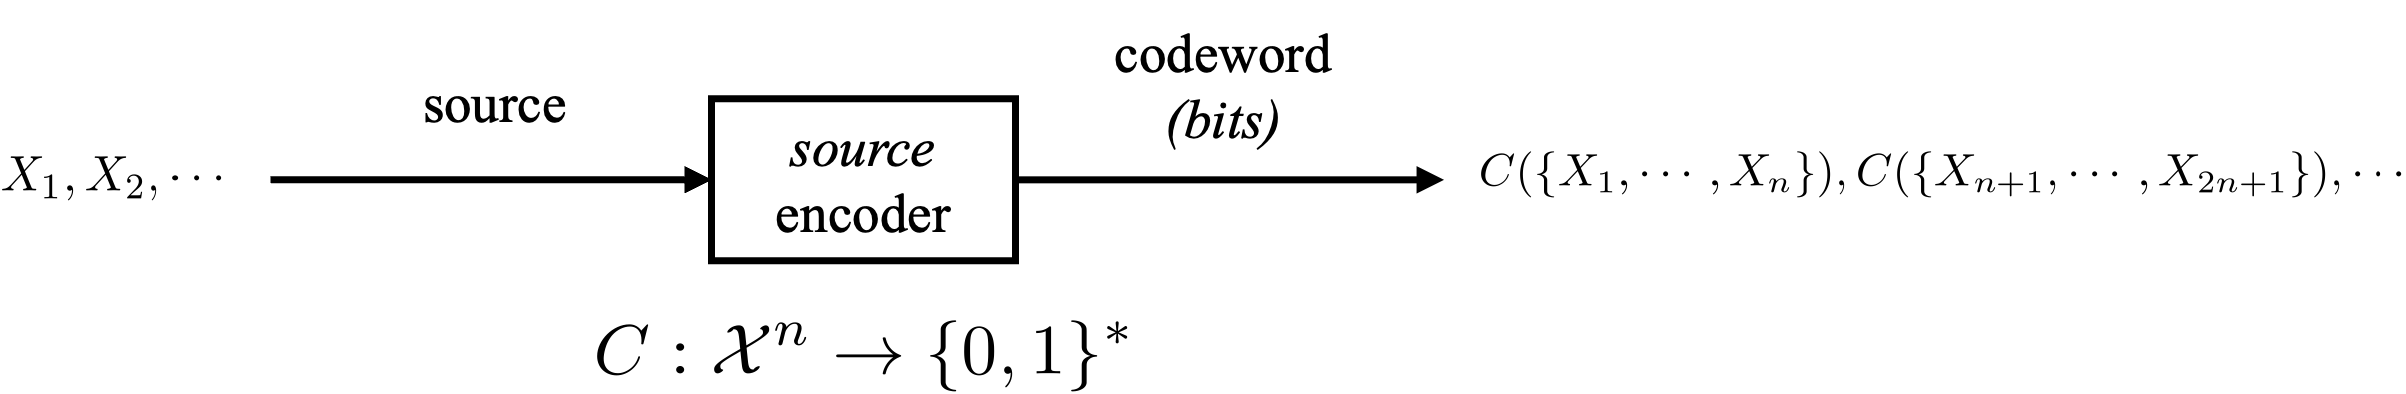
\includegraphics[width=0.9\columnwidth]{image/L3_block.png}
            \end{figure}
            \begin{itemize}
                \item Block code를 사용했을 때, 각 symbol에 대한 code word length의 기댓값 $R_n$은 다음과 같이 계산할 수 있다.
                $$R_n = \frac{1}{n} \sum_{x^n \in \mathcal X^n} p(x^n) \cdot l(x^n)\qquad \text{(bits/source)}$$
                \item 특정 rate $R$을 이용하는 fixed length block code의 encoder, decoder는 다음과 같이 표현된다.
                $$ \begin{aligned} & f_n: X^n \rightarrow\{0,1\}^{n R}=\big\{0,1, \cdots, 2^{nR}-1 \big\} 
                    \\ & g_n:\{0,1\}^{n R} \rightarrow X^n \end{aligned} $$
            \end{itemize}
        \end{frame}
        
        \begin{frame}
            \frametitle{Lossless source coding}
            \begin{itemize}
                \item block coding은 source data의 \textit{sequence}를 다루기 때문에, sample space가 exponential하게 커진다. 
                \item 만약, sample space의 모든 데이터에 대하여 one-to-one mapping을 사용하여 encoding을 하게 되면 decoding에서 error는 발생하지 않지만, codeword의 길이가 너무 길어진다.
                $$ |\mathcal X |^n \le 2^{nR},\quad nR \ge \lceil \log |\mathcal X |^n \rceil$$
                \item 따라서 약간의 error는 허용하고 codeword의 길이를 효율적으로 줄이기 위한 방법을 \textbf{lossless source coding}이라고 한다.
            \end{itemize}
            \begin{definition}
                The probability of error source code scheme is defined as  $$ P_e^{(n)} \triangleq P^n\left(\left\{x^n: g_n\left(f_n\left(x^n\right)\right) \neq x^n\right\}\right) $$
            \end{definition}
        \end{frame}

        \begin{frame}
            \frametitle{Lossless source coding}
            lossless source coding에서 error는 $n$이 증가함에 따라서 \alert{0으로 수렴}해야한다.
            
            \begin{definition}
                For any $\epsilon>0$, we say a rate $R$ is an \textbf{achievable rate} of source coding for with probability of error $\epsilon$, if there exists a sequence of $(n, R)$ codes such that
                $$ \limsup _{n \rightarrow \infty} P_e^{(n)} \leq \epsilon $$
            \end{definition}

            \begin{definition}
                The \textbf{minimum of such rates} for a given $\epsilon$ is denoted as $R_{\min}(\epsilon)$, which is the achievable source coding rate allowing error probability $\epsilon$. We further define 
                $$ R_{\min }=\lim _{\epsilon \rightarrow 0} R_{\min }(\epsilon) $$
            \end{definition}
        \end{frame}


        \begin{frame}
            \frametitle{Lossless source coding theorem}
            \begin{theorem}[Lossless Source Coding Theorem]
                The minimum achievable rate of lossless source coding for DMS ( $P$ ) is 
                $$ R_{\min }=H(P) \text {. } $$
            \end{theorem}
            \vspace{0.2cm}
            Lossless source coding theorem은 \textit{Achievability}, 그리고 \textit{Converse}의 2가지 성질을 모두 가지며, 두 upper bound와 lower bound가 동일한 complexity $O(H(P))$를 가지므로 최적의 solution이다. 
            \vspace{0.2cm}
            \begin{itemize}
                \item Achievability: 만약 $R > R_{\min} = H(P)$인 rate를 사용한다면, probability of error가 0으로 수렴하는; $\lim_{n\rightarrow \infty} P_{e}^{(n)} = 0$ sequence of $(n, R)$ code가 존재한다.
                \item Converse: 만약 $R < R_{\min} = H(P)$인 rate를 사용한다면, 그 어떤 code scheme도 probability of error가 0으로 수렴함을 보장하지 못한다. 
            \end{itemize}
        \end{frame}


        \begin{frame}
            \frametitle{Proof of lossless source coding theorem: achievable}
            $\ast$ \underline{Proof}: (hint) Weak typical set
            \vspace{0.2cm}
            \begin{itemize}
                \item Weak typical set 안에 있는 data에 대한 one-to-one mapping scheme를 고려하자. Weak typical set의 크기는 다음과 같이 bound된다.
                $$ |A_{\delta}^{(n)} (P)| \le 2^{n(H(P)+\delta)}$$
                \item 이때, $R > H(P)$인 rate를 사용한다고 생각하자. 그럼 항상 우리는 다음과 같은 $\delta$를 고려할 수 있다.
                $$R > H(P) + \delta > H(P)$$
                \item error는 source data가 typical set안에 존재하지 않을 때만 발생하기 때문에, 다음과 같다.
                $$P^{(n)}_{\epsilon} \ge 1- \epsilon$$
                \item 따라서 WLLN에 의해 if $n \rightarrow \infty$, then
                $$ P^{(n)}_{\epsilon} \rightarrow 0.$$
            \end{itemize}
        \end{frame}

        \begin{frame}
            \frametitle{Proof of lossless source coding theorem: converse}
            $\ast$ \underline{Proof}: (hint) Fano's inequality
            \vspace{0.2cm}
            \begin{itemize}
                \item Source coding에서 decoding은 fano's inequality의 experiment로 생각할 수 있다.
                \begin{itemize}
                    \item $X^n$: 원본 source data
                    \item $Y=f_n(X^n)$: encoder
                    \item $\hat X = g_n(Y)$: decoder 
                    \item $P_e^{(n)} = P(g_n(Y) \ne X^n)$: error probability
                \end{itemize}
                \item 따라서 Fano's inequality를 이용하여 전개하면 다음과 같고
                \begin{align*} 
                nH(P) = H(X^n) &= H(X^n | Y) + I(X^n ; Y)\\
                &\le \qquad \qquad \qquad \qquad \qquad \qquad \qquad \qquad \qquad \qquad\\
                &\le \\
                &\le
                \end{align*}
                \item error probability에 대해 정리하면 다음과 같다.
                \begin{itemize}
                    \item if $R<H(P)$: $\lim_{n \rightarrow \infty}$일 때, 0으로 수렴하지 않는다.
                    \item if $R>H(P)$: $\lim_{n \rightarrow \infty}$일 때, 0으로 수렴한다.
                \end{itemize}
                $$
                P_e^{(n)} \geq \frac{H(P)-R-\frac{1}{n}}{\log |\mathcal{X}|}
                $$
                \item 따라서, $n\rightarrow \infty$일 때, $P^{(n)}_\epsilon \rightarrow 0$을 만족하기 위해서는 $R \ge H(P)$여야한다.$\Box$  % necessary condition of lossless source coding
            \end{itemize}
        \end{frame}

        \begin{frame}
            \frametitle{Summary}
            \textit{Some Remarks}
            \begin{itemize}
                \item Operation meaning of $H(P)$
                \begin{itemize}
                    \item 원래 entropy는 $X \sim P$에 대해 realization value $x$를 알았을 때, 얻게되는 정보량에 대한 average를 의미한다.
                    \item data compression의 관점에서 생각하면, $n\rightarrow \infty$에 따라 $nH(P)$ bits가 lenght $n$ sequence를 표현하기 위한 bits의 개수가 된다.
                \end{itemize}
                \item Variable-length block code
                \begin{itemize}
                    \item Variable length coding 방식을 이용하면 $nH(P)$보다 더 작은 길이의 encoding scheme을 설계할 수 있는가? $\rightarrow$ 불가능
                    \item typical set 내부의 data들의 확률은 거의 동일하기 때문에, Huffman algorithm 같은 방식을 도입해도 길이가 비슷하다.
                \end{itemize}
                \item Optimal uniquely decodable code $P_\epsilon ^{(n)}=0$
                \begin{itemize}
                    \item (prefix-code)  typical set 내부에 있는 data는 0으로 시작하는 bit-string과 mapping하고 typical set 외부에 있는 data는 1로 시작하는 bit-string과 mapping한다.
                    \item average rate 다음과 같기 때문에, $n\rightarrow \infty$에 따라서 $R\rightarrow H(P)$로 수렴한다.
                    $$ nR = P^n(A_\epsilon^{(n)}(P)) \cdot(1+nH(P)) +  P^n(A_\epsilon^{(n)}(P)^c) \cdot(1+n \log|\mathcal X|) $$
                \end{itemize}
            \end{itemize}
        \end{frame}

    \end{section}

    \begin{frame}{References}
        \begin{itemize}
            \item T. M. Cover and J. A. Thomas. Elements of Information Theory, Wiley, 2nd ed., 2006.
            \item Gallager (2008), Principles of Digital Communication, Cambridge University Press.
            \item Lecture notes for EE623: Information Theory (Fall 2024)
        \end{itemize}
        \vspace{6cm}
    \end{frame}


\end{document}